% *********************************************************************
% © 2021 Jeremy Sylvestre
%
% Permission is granted to copy, distribute and/or modify this document
% under the terms of the GNU Free Documentation License, Version 1.3 or
% any later version published by the Free Software Foundation; with no
% Invariant Sections, no Front-Cover Texts, and no Back-Cover Texts. A
% copy of the license is included in the appendix entitled “GNU Free
% Documentation License” that appears in the output document of this
% PreTeXt source code. All trademarks™ are the registered® marks of
% their respective owners.
%
% *********************************************************************

\newcommand*{\xmin}{-6}
\newcommand*{\xmax}{42}
\newcommand*{\ymin}{-10}
\newcommand*{\ymax}{110}

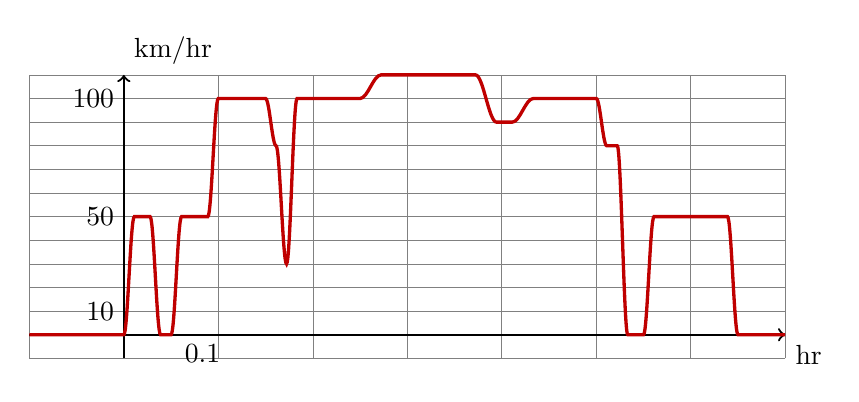
\begin{tikzpicture}
[
	closedpt/.style={circle,draw,fill,inner sep=0pt,minimum size=4pt},
	openpt/.style={circle,draw,inner sep=0pt,minimum size=4pt},
	xscale=0.2,
	yscale=0.03
]

	% grid
	\foreach \x in {-6,0,6,...,42} {
		\draw[very thin,gray] (\x,\ymin) -- (\x,\ymax);
	}
	\foreach \y in {-10,0,10,...,110} {
		\draw[very thin,gray] (\xmin,\y) -- (\xmax,\y);
	}

	% label grid
	\node[below] at (5,0) {$0.1$};
	\foreach \y in {10,50,100} {
		\node[left] at (0,\y) {$\y$};
	}

	% axes
	\draw[->,thick] (\xmin,0) -- (\xmax,0) node[below right] {hr};
	\draw[->,thick] (0,\ymin) -- (0,\ymax) node[above right] {$\mathrm{km}/\mathrm{hr}$};

	% continuous graph
	\draw[red!75!black,very thick]
	  (\xmin,0) -- (0,0)
	  cos ( 0.333,  25)
	  sin ( 0.667,  50)
	  --  ( 1.667,  50)
	  cos ( 2.000,  25)
	  sin ( 2.333,   0)
	  --  ( 3.000,   0)
	  cos ( 3.333,  25)
	  sin ( 3.667,  50)
	  --  ( 5.333,  50)
	  cos ( 5.667,  75)
	  sin ( 6.000, 100)
	  --  ( 9.000, 100)
	  cos ( 9.333,  90)
	  sin ( 9.667,  80)
	  cos (10.000,  55)
	  sin (10.333,  30)
	  cos (10.667,  65)
	  sin (11.000, 100)
	  --  (15.000, 100)
	  cos (15.667, 105)
	  sin (16.333, 110)
	  --  (22.333, 110)
	  cos (23.000, 100)
	  sin (23.667,  90)
	  --  (24.667,  90)
	  cos (25.333,  95)
	  sin (26.000, 100)
	  --  (30.000, 100)
	  cos (30.333,  90)
	  sin (30.667,  80)
	  --  (31.333,  80)
	  cos (31.667,  40)
	  sin (32.000,   0)
	  --  (33.000,   0)
	  cos (33.333,  25)
	  sin (33.667,  50)
	  --  (38.333,  50)
	  cos (38.667,  25)
	  sin (39.000,   0)
	  --  (\xmax,    0)
	;

\end{tikzpicture}
